\section{Evaluation} \label{sec:evaluation}

\begin{table}[b]
\footnotesize
\centering
\vspace{-.15in}
\begin{tabular}{lrr}
{\bf Program} & {\bf Benchmark} & {\bf Workload/input description}\\
\hline\\[-2.3ex]
\clamav & clamscan~\cite{clamscan}  & Files in \v{/lib} from a replica \\
\mediatomb & ApacheBench~\cite{apachebench}  & Transcoding videos\\
\memcached & mcperf~\cite{mcperf}  & 50\% set, 50\% get operations\\
\mongodb & YCSB~\cite{ycsb}  & Insert operations\\
\mysql & Sysbench~\cite{sysbench}  & SQL transactions\\
\openldap & Self  & LDAP queries\\
\redis & Self  & 50\% set, 50\% get operations\\
\ssdb & Self  & Eleven operation types\\
\calvin & Self  & SQL transactions\\
\end{tabular}
\vspace{-.05in}
\caption{{\em Benchmarks and workloads.} ``Self" in the Benchmark column means 
we used a program's own performance benchmark program. Workloads are all 
concurrent.} 
\label{tab:benchmarks}
\end{table}

\begin{figure*}[t]
\centering
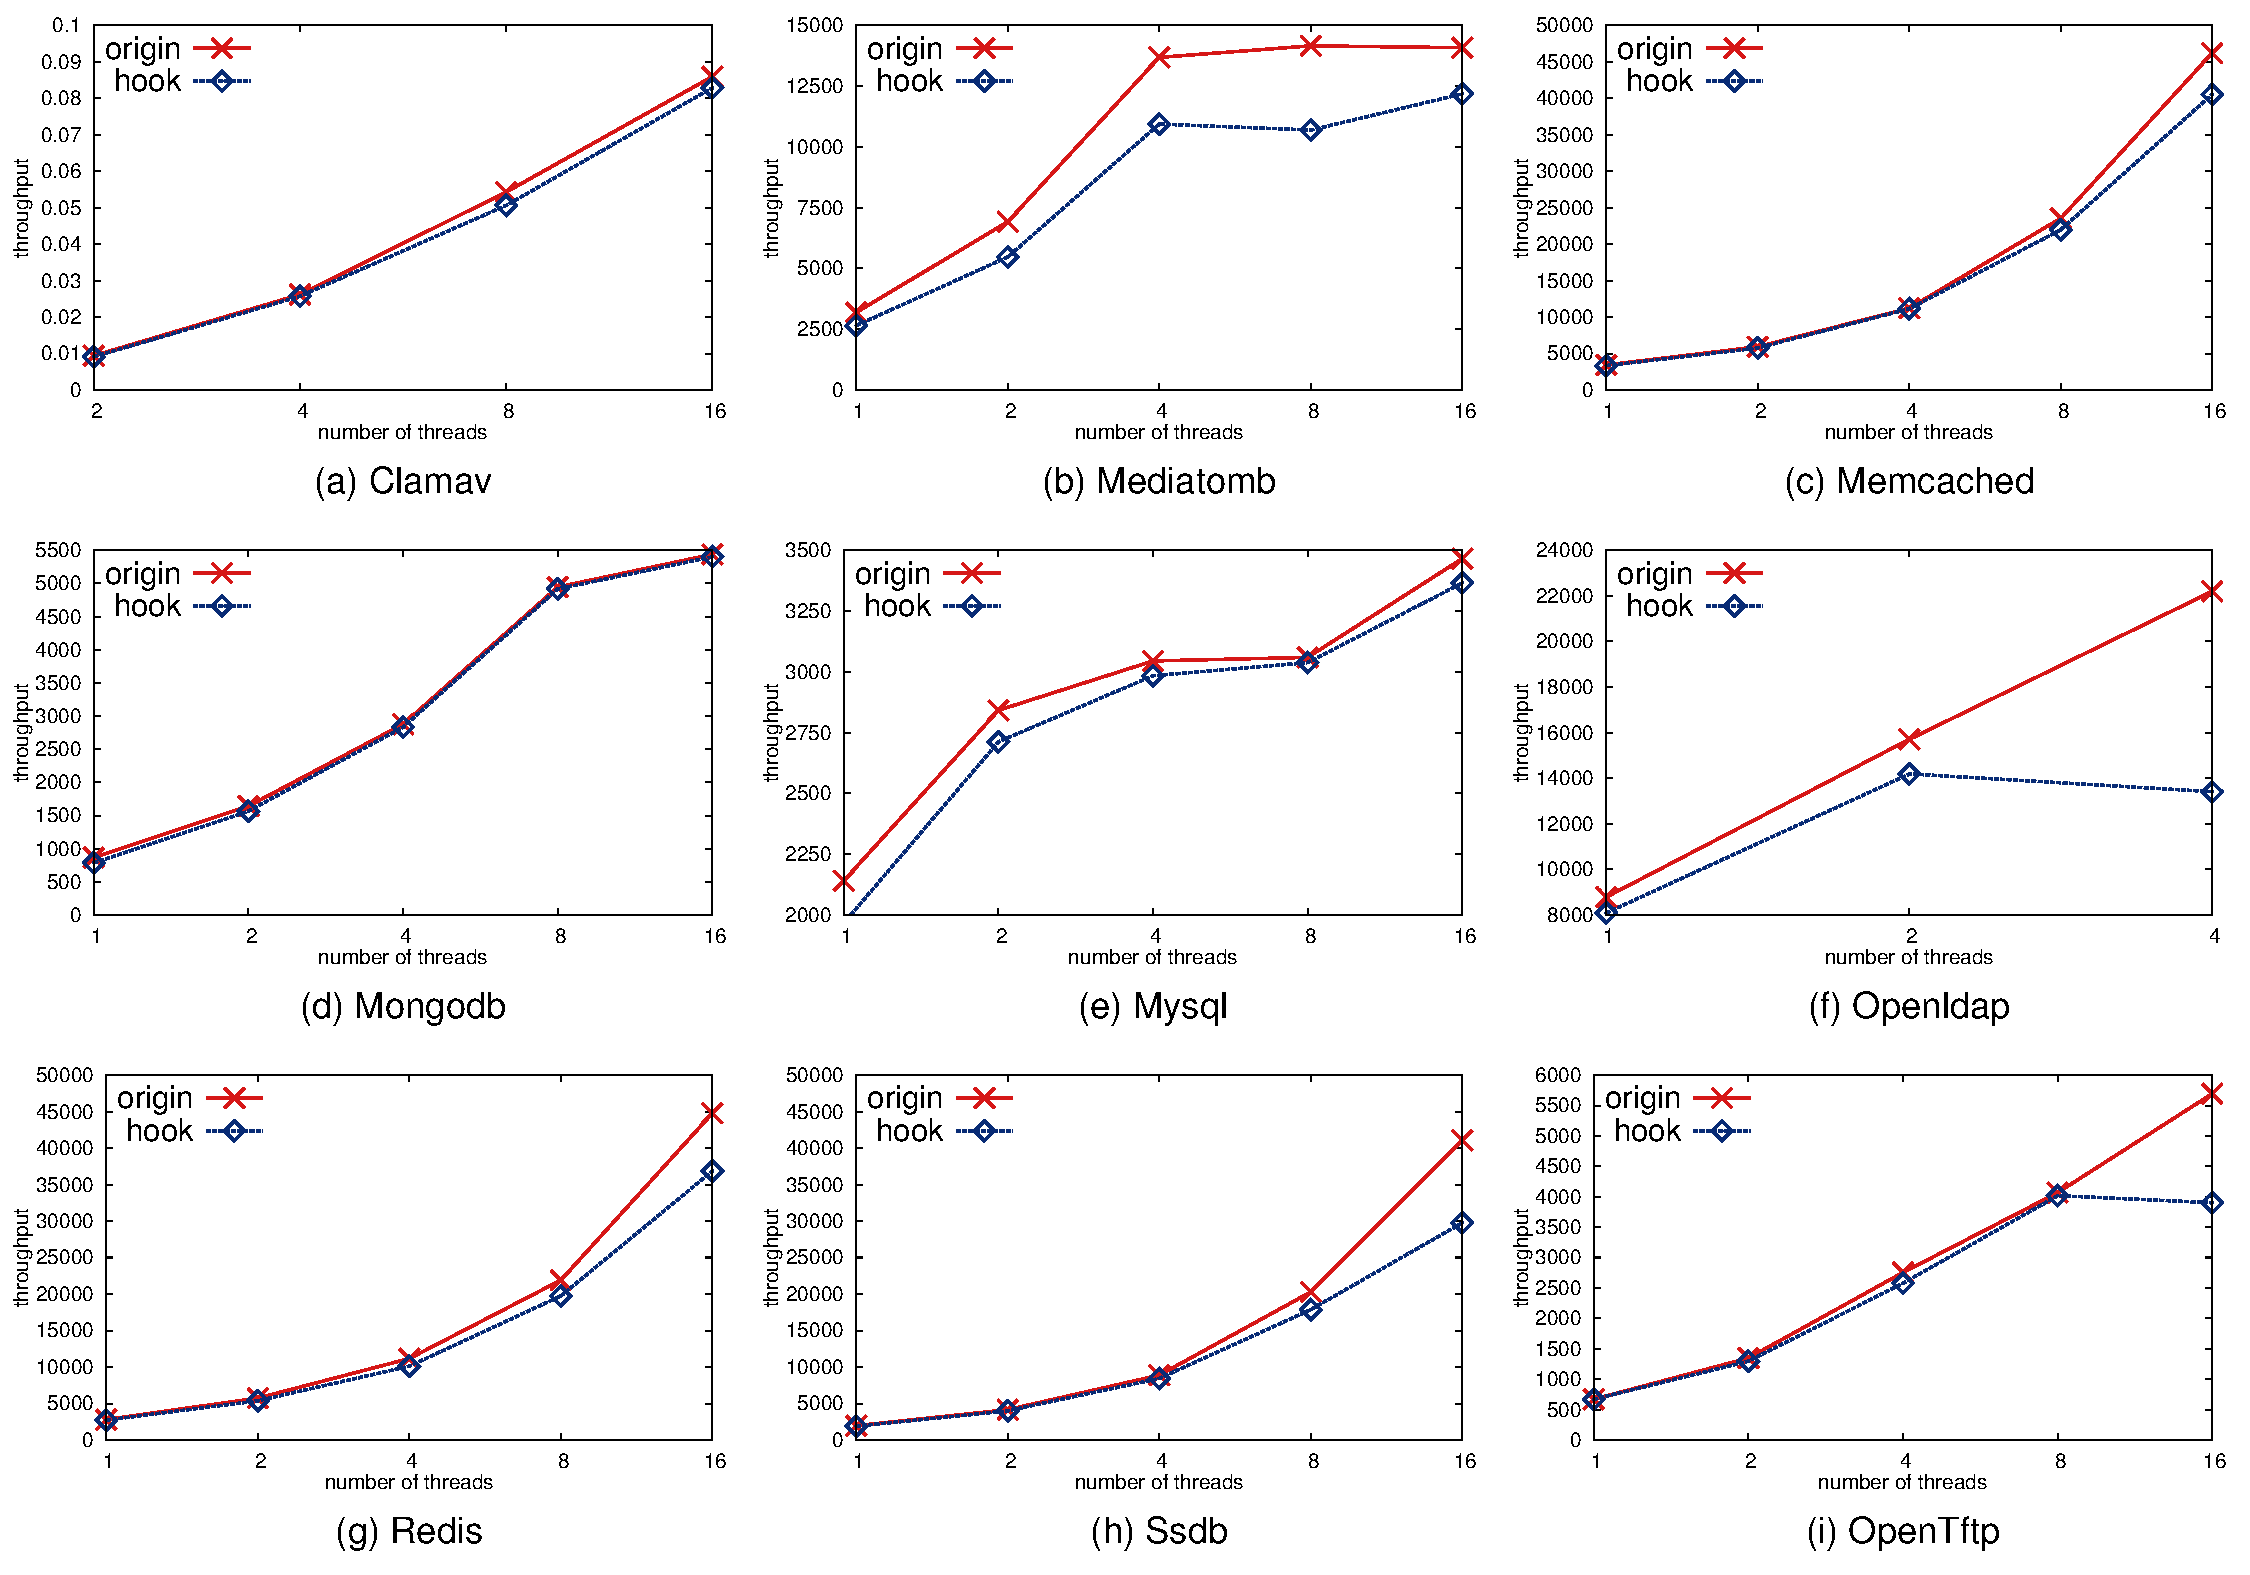
\includegraphics[width=0.9\textwidth]{figures/throughput}
\vspace{-.10in}
\caption{\small {\em \xxx throughput compared to the unreplicated 
execution.}}
\vspace{-.20in}
\label{fig:tput}
\end{figure*}

\begin{figure*}[t]
\centering
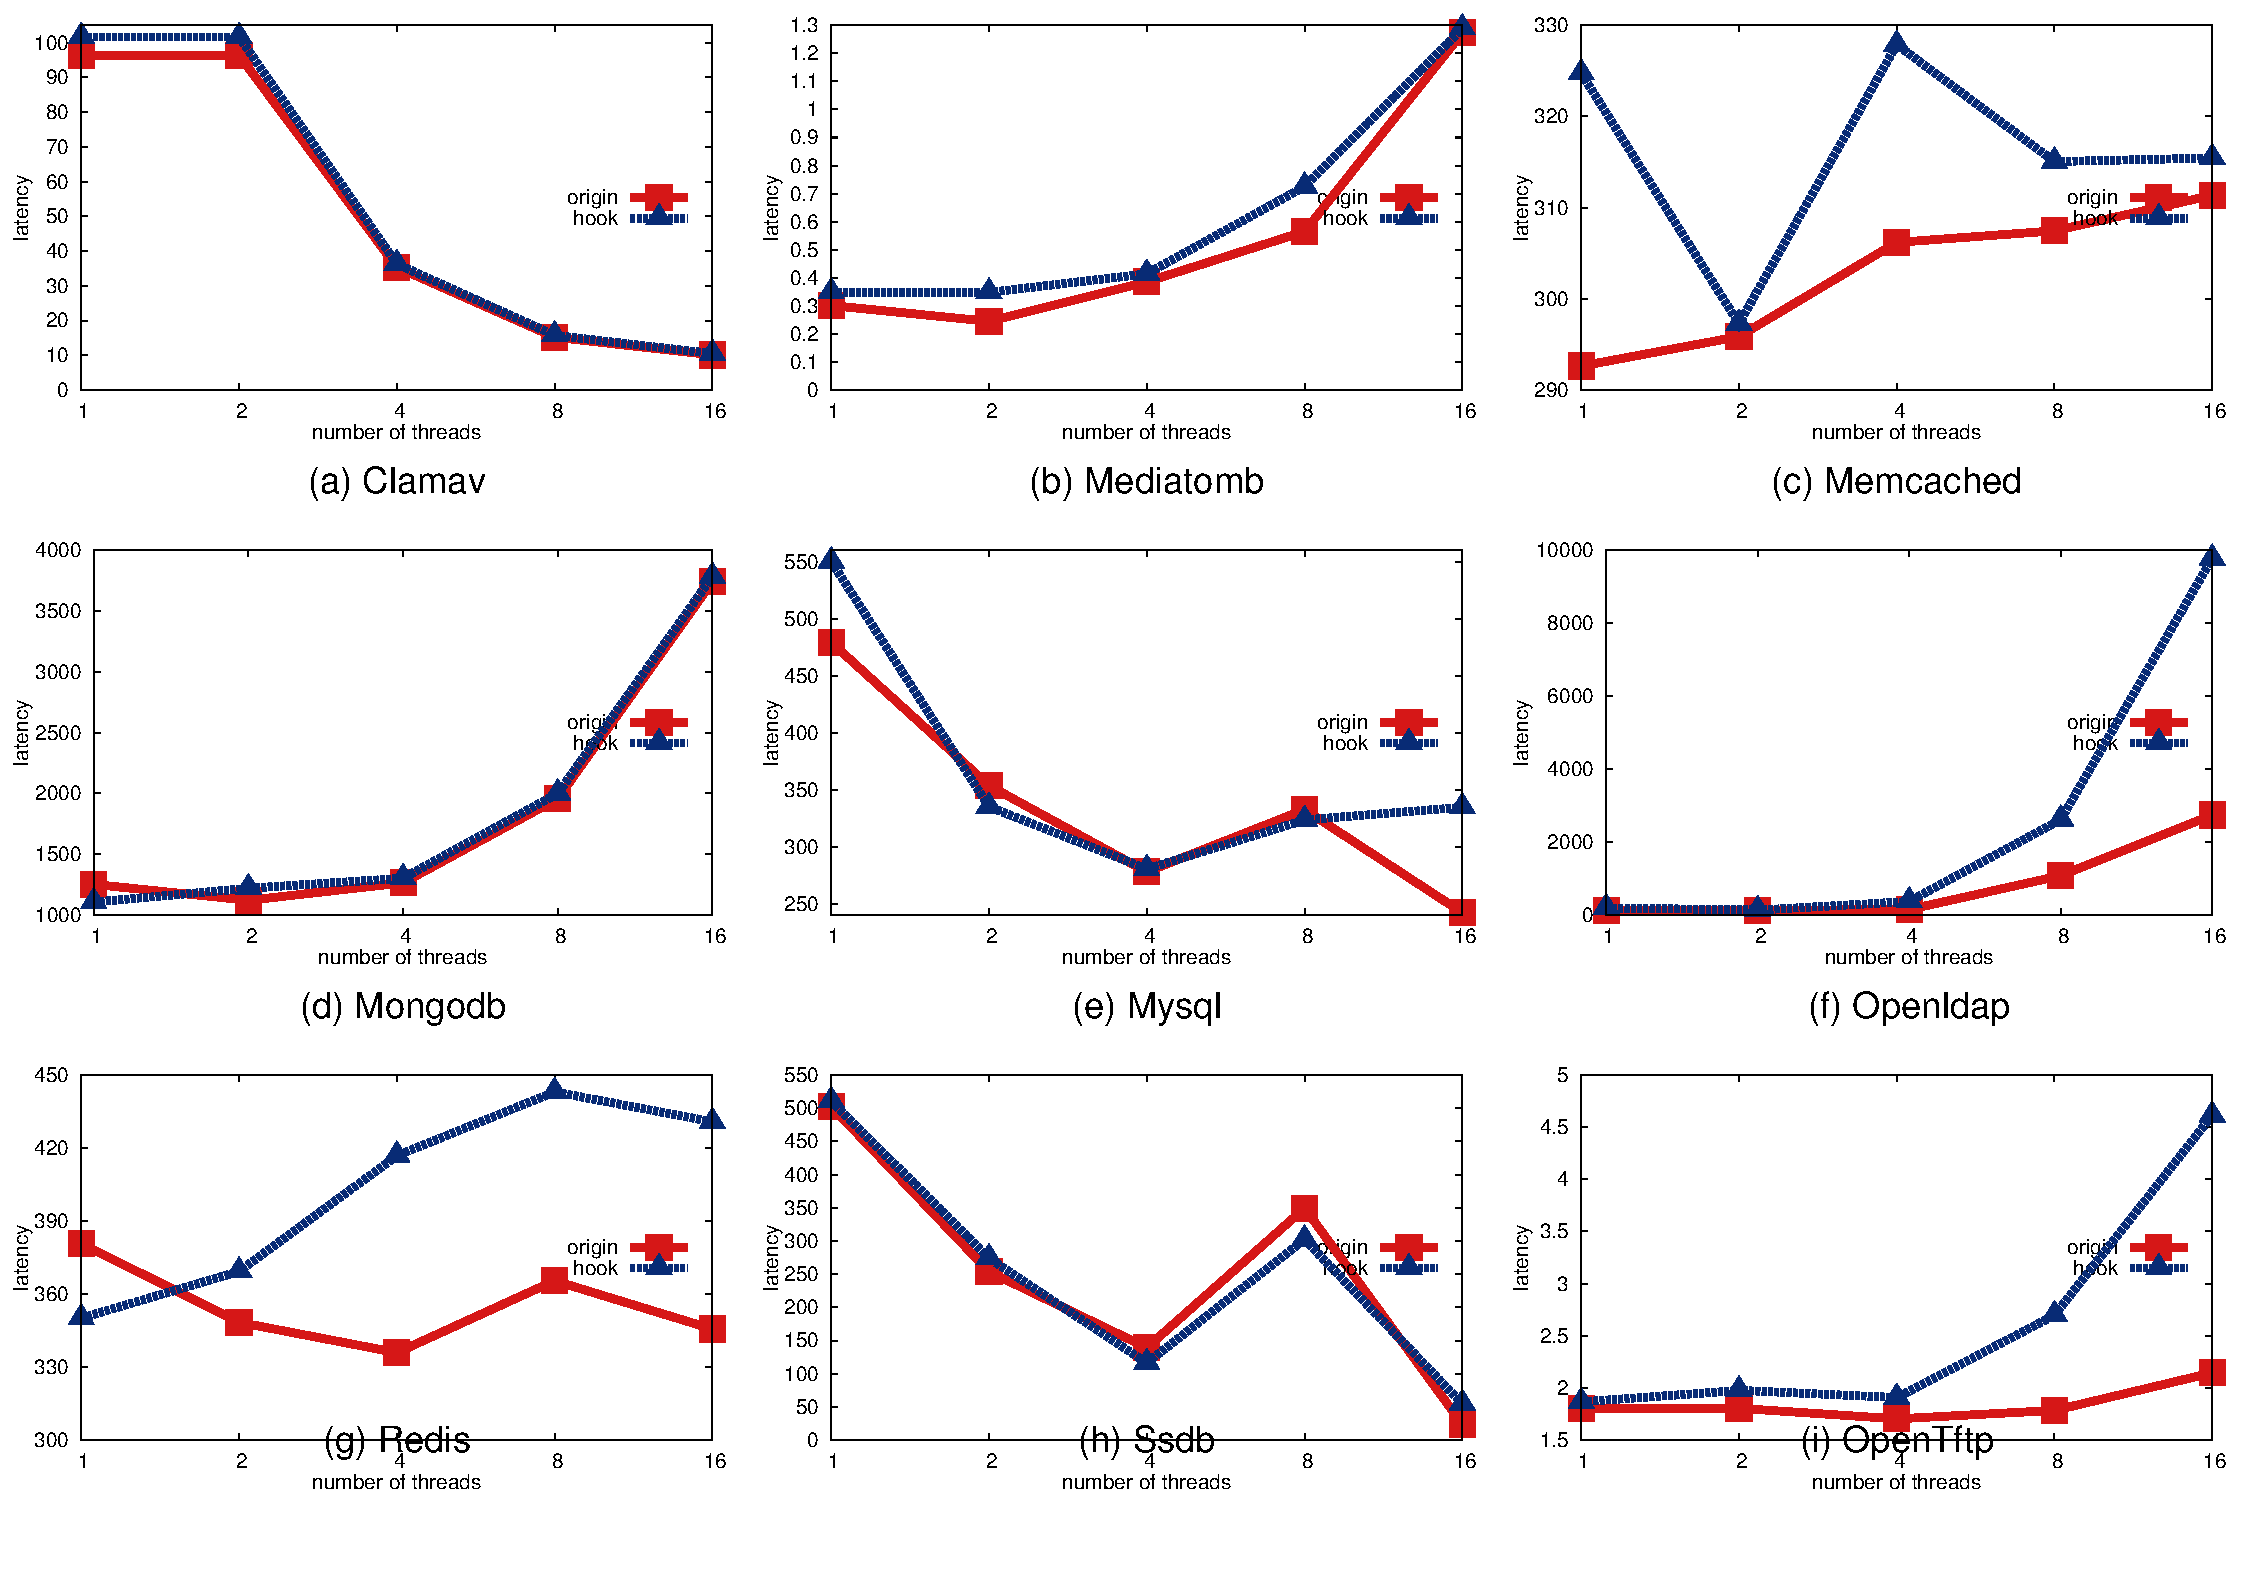
\includegraphics[width=0.9\textwidth]{figures/latency}
\vspace{-.10in}
\caption{\small {\em \xxx response time compared to the unreplicated 
execution.}}
\vspace{-.20in}
\label{fig:latency}
\end{figure*}

Our evaluation used three Dell R430 servers as SMR replicas. Each server having 
Linux 3.16.0, 2.6 GHz Intel Xeon CPU with 24 hyper-threading cores, 64GB 
memory, and 1TB SSD. Each machine has a Mellanox ConnectX-3 Pro Dual Port 40 
Gbps NIC. These NICs are connected using the Infiniband RDMA architecture 
through a Dell S6000 high-performance switch with 32 40Gpbs ports. The \v{ping} 
latency between every two replicas are 84 \us (the IPoIB round-trip latency).

To mitigate network latency of public network, all client benchmarks were ran 
in a Dell R320 server (the client machine), with Linux 3.16.0, 2.2GHz Intel 
Xeon with 12 hyper-threading cores, 32GB memory, and 160GB SSD. This server 
connects with the replica machines with 1Gbps bandwidth LAN. The average 
\v{ping} latency between the client machine and a replica machine is 301 \us. A 
larger network latency (\eg, sending client requests from WAN) will further 
mask \xxx's overhead.

We evaluated \xxx on \nprog widely used or studied server programs, including 
\nkvprog key-value stores \redis, \memcached, \ssdb, \mongodb; \mysql, a SQL 
server; \clamav, a anti-virus server that scans files and delete malicious ones; 
\mediatomb, a multimedia storage server that stores and transcodes video and 
audio files; \openldap, an LDAP server; \calvin, a widely studied transactional 
database system that leverages \zookeeper as its SMR service. All these programs 
are multithreaded except \redis (but it can serve concurrent requests via 
Libevent). These servers all update or store important data and files, thus the 
strong fault-tolerance of SMR is especially attractive to these programs.

% Benchmarks table.
Table~\ref{tab:benchmarks} introduces the benchmarks and workloads we used. To 
evaluate \xxx's practicality, we used the server developers' own performance 
benchmarks or popular third-party. For benchmark workload settings, we used the 
benchmarks' default workloads whenever available. We spawned up to 16 
concurrent connections, and then we measured both response time and 
throughput. We also measured \xxx's bare consensus latency. All evaluation 
results were done with a replica group size of three except the scalability 
evaluation (\S\ref{sec:scalability}). Each performance data point in the 
evaluation is taken from the mean value of 10 repeated executions.

% evaluation metric. client benchmarks all run in LAN, average latency
The rest of this section focuses on these questions:

\begin{tightenum}

\item[\S\ref{sec:ease-of-use}:] Is it easy to run general server programs 
in \xxx?

\item[\S\ref{sec:overhead}:] What is \xxx's performance compared to the 
unreplicated executions? What is the consensus latency of \xxx's \paxos 
protocol?

\item[\S\ref{sec:scalability}:] How scalable is \xxx on different replica group 
sizes?

\item[\S\ref{sec:compare}:] What is \xxx's performance compared to existing 
SMR systems?

\item[\S\ref{sec:robust}:] How fast can \xxx checkpoint and recover replicas 
when output divergence is detected?

% \item[\S\ref{sec:race}:] If some \xxx users care about data races much, how 
% does \xxx tolerate the slowdown of data race detector by deploying it on a 
% replica?

% \item[\S\ref{sec:lesson}:] What practical lessons have we learnt during the 
% case study on these server programs with \xxx?

\end{tightenum}


\subsection{Ease of Use} \label{sec:ease-of-use}

\xxx is able to run all \nprog evaluated programs without modifying them except 
\calvin. \calvin integrates its client program and server program within the 
same process and uses local memory to let these two programs communicate. To 
make \calvin's client and server communicate with POSIX sockets so that \xxx 
can intercept the server's inputs, we wrote a \nlinescalvin patch for \calvin.

\subsection{Performance Overhead} \label{sec:overhead}

Figure~\ref{fig:tput} shows \xxx's throughput and Figure~\ref{fig:latency} 
response time. We varied the number of concurrent client connections for each 
server program by from one to 16 threads. For \calvin, we only collected the 
8-thread result because \calvin uses this constant thread count in their code 
to serve client requests. Overall, compared to these server programs' 
unreplicated executions, \xxx merely incurred a mean throughput degrade by 
\tputoverhead (note that in Figure~\ref{fig:tput}, the Y-axises of most programs 
start from a large number). \xxx's mean overhead on response time was merely 
\latencyoverhead.

As the number of threads increases, all programs' unreplicated executions 
got a performance improvement except \memcached. A prior 
evaluation~\cite{rex:eurosys14} also observed a similar \memcached low 
scalability. \xxx scaled almost as well as the unreplicated executions.
% a \latencyoverhead overhead compared to the unreplicated 
% executions.

\xxx achieves such a low overhead in both throughput and response time mainly 
because of two reasons. First, for each \recv call in a server, \xxx's input 
coordination protocol only contains two one-sided RDMA writes and two SSD writes 
between each leader and backup. A parallel SSD write 
approach~\cite{Bessani:usenix13} may further improve \xxx's SSD performance.  
Second, \xxx's output checking protocol, which is based on the input 
coordination protocol, invokes occasionally, once for every \thashcomp output 
hash generations (\S\ref{sec:output-workflow}).

\begin{table}[h]
\footnotesize
\centering
\vspace{.05in}
\begin{tabular}{lrrrr}
{\bf Program} & {\bf \# Calls} & {\bf Input} & {\bf SSD time} 
& {\bf Quorum time}\\
\hline\\[-2.3ex]
% Heming: normalized clamav to 10K req.
\clamav & 30,000  & 42.0 & 4.9 \us & 7.2 \us\\
% TBD: normalize mediatomb to 10K req.
\mediatomb & 30,000  & 140.0 & 4.4 \us & 6.9 \us\\
\memcached & 10,016  & 38.0 & 4.6 \us & 6.3 \us\\
\mongodb & 10,376  & 492.4 & 14.9 \us & 16.4 \us\\
\mysql & 10,009  & 26.0 & 5.0 \us & 8.4 \us\\
% TBD: normalize ldap to 10K req.
\openldap & 10,016  & 27.3 & 6.4 \us & 12.0 \us\\
\redis & 10,016  & 107.0 & 3.6 \us & 6.3 \us\\
% TBD: normalize ssdb to 10K req.
\ssdb & 10,016  & 47.0 & 3.7 \us & 10.9 \us\\
\calvin & 10,002  & 93.0 & 2.5 \us  & 9.9 \us\\
\end{tabular}
\vspace{-.05in}
\caption{{\em Leader's input consensus events per 10K requests, 8 threads.} 
The ``\# Calls" column means the number of socket calls that went through \xxx 
input consensus; ``Input" means average bytes of a server's inputs received in 
these calls; ``SSD time" means the average time spent on storing these calls to 
stable storage; and ``Quorum time" means the average time spent on waiting 
quorum for these calls.} 
\label{tab:consensus-latency}
\end{table}

% Figure~\ref{fig:latency} shows \xxx's latency.
% % Bare consensus latency, micro events.

To deeply understand \xxx's performance overhead, we collected the number of 
socket call events and consensus durations in the leader replica. 
Table~\ref{tab:consensus-latency} shows these statistics per 10K requests, 8 
or max (if less than 8) threads. According to the consensus algorithm steps in 
Figure~\ref{fig:consensus}, for each socket call, \xxx's leader does an ``L2": 
SSD write (the ``SSD time" column in Table~\ref{tab:consensus-latency}) and an 
``L4": quorum waiting phase (the ``quorum time" column). L4 implies backups' 
performance because each backup stores the proposed socket call in local SSD and 
then WRITEs a consensus reply to the leader.

By summing these two time columns, overall, a \xxx input consensus took only 
9.9 \us (\redis) to 39.6 \us (\mongodb). This consensus latency mainly depends 
on the ``Input" column: the average number of data bytes received in socket 
calls (\eg, \mongodb has the largest received bytes). \xxx's small consensus 
latency makes \xxx achieve reasonable throughputs in Figure~\ref{fig:tput} and 
response times Figure~\ref{fig:latency}. This small latency suggests that, even 
if clients are deployed within the same datacenter network, \xxx may still 
achieve acceptable overhead on many programs (although \xxx's deployment 
model is running server replicas in a datacenter and clients in LAN 
or WAN).

\subsection{Comparison with Other SMR systems} \label{sec:compare}

We compared \xxx with \calvin's SMR system because \calvin's input consensus 
uses \zookeeper, one of the most widely used coordination service built on 
TCP/IP. To conduct a fair comparison, we ran \calvin's own transactional 
database server in \xxx as the server program, and we compared throughputs and 
the consensus latency with \calvin's consensus protocol \zookeeper.

As shown in Table~\ref{tab:compare}, \calvin's \zookeeper replication achieved 
19.9K transactions/s with a 511.9 \us consensus latency. \xxx achieved 17.6K 
transactions/s with a 12.5 \us consensus latency. The throughput in \calvin 
was 13.1\% higher than that in \xxx because \calvin puts transactions in a 
batch with a 10 \ms timeout, it then invokes \zookeeper for consensus on 
this batch. The average number of bytes in \calvin's batches is 18.8KB, and 
the average number of input bytes in each \xxx consensus (one for each \myread 
call) is 93 bytes. Batching helps \calvin achieve good throughput. \xxx 
currently has not incorporated a batching technique because its latency is 
already reasonable (\S\ref{sec:overhead}).

Notably, \xxx's consensus latency was 40.1X faster than \zookeeper's mainly due 
to \xxx's RDMA-accelerated consensus protocol, although we ran \calvin's 
\zookeeper consensus on IPoIB. A prior SMR evaluation~\cite{dare:hpdc15} also 
reports a similar 320 \us consensus latency in \zookeeper. Two other recent SMR 
systems Crane~\cite{crane:sosp15} and Rex~\cite{rex:eurosys14} may incur similar 
consensus latency as \zookeeper's because all their consensus protocols are 
based on TCP/IP. Overall, this \xxx-\calvin comparison suggests that \calvin 
will be better if clients prefer high throughput, and \xxx will be better if 
clients demand short latency.

\begin{table}[t]
\footnotesize
\centering
% \vspace{-.2in}
\begin{tabular}{lrr}
{\bf Performance metric} & {\bf \zookeeper} & {\bf \xxx}\\
\hline\\[-2.3ex]
Throughput (requests/s) & 19,925   & 17,614 \\
Consensus latency (\us) & 511.9  & 12.5\\
\end{tabular}
\vspace{-.1in}
\caption{{\em Comparison with \calvin's \zookeeper replication.}} 
\vspace{-.2in}
\label{tab:compare}
\end{table}





% Comparison with Crane. Run Crane. TBD


\subsection{Scalability on Replica Group Size} \label{sec:scalability}

% TBD: rerun \redis micro events; it is too small, so we can not use it here.

Because we had only three RDMA-enable machines in the evaluation time, we 
picked \redis as the testing program and ran five to seven \xxx instances on 
three machines: one machine held the leader instance, and each of the other two 
to three machines held two backups.

Given the same \redis workload, \xxx's five-replica setting had a 17.9K 
requests/s and 10.1 \us consensus latency, and its seven-replica setting had a 
17.4K requests/s and 11.0 \us consensus latency. Compared to the three-replica 
setting, 18.0K throughput and 9.9 \us consensus latency, \xxx achieves a similar 
consensus latency from three to seven replicas, which mainly depends on the 
latency of two SSD stores and one WRITE round-trip (see 
Table~\ref{tab:consensus-latency}).

We didn't consider these initial scalability results general; we found them 
promising. Given that each RDMA NIC hardware port supports up to 16 outbound 
RDMA WRITEs with peak performance~\cite{herd:sigcomm14}, and our NIC has dual 
ports, we anticipate that our algorithm may scale up to around 32 replicas 
under current hardware techniques. We plan to buy more RDMA servers and verify 
whether \xxx's scalability is bounded by the capacity of RDMA hardware.


% For seven nodes 
% XXX TBD. We plan to buy more server machines for a larger scale of scalability 
% evaluation.

% It 
% would be interesting to see whether \xxx's scalability on replica group size is 
% bounded by the outbound RDMA writes of RDMA NICs.



% Comparison with DARE. Three to five nodes.

\subsection{Checkpoint and Recovery} \label{sec:robust}

For all the \nprog programs, our output checking protocol found these servers 
produced identical results except \clamav and \mediatomb. The output divergence 
of \clamav is because its threading model. \clamav uses multiple threads to 
serve a directory scan request, where the threads scan files in parallel and 
append the scanned files into a shared output buffer protected by a mutex lock. 
Therefore, sometimes \clamav's output will diverge across replicas. Attaching a 
deterministic multithreading runtime with \clamav avoided this 
divergence~\cite{crane:sosp15}. \mediatomb contained physical timestamp in its 
replies. \calvin did not send outputs to its client.

% TBD: what types of servers are good for output checking.

Each \xxx periodic checkpoint operation cost between 0.12s to 11.6s to the 
evaluated server programs. The checkpoint duration depends on whether a 
server's process has read files in its memory or modified files in its current 
working directory. \clamav incurred the largest checkpoint time (11.6s) because 
we ran it to scan files with a total size of $\sim$3GB in a \v{/lib} directory. 
We ran our recovery mechanism to recover \clamav from its diverged 
timestamps, which rollbacks of all three replicas. A \clamav rollback time 
varied from 0.81s to 2.72s for backups and the leader, including extracting a 
checkpoint ZIP, restoring process state with CRIU, and reconnecting RDMA QPs 
with remote replicas.



% Heming: TBD, just estimation. Current 0.81s to 2.72s are from redis.





\begin{table}[h]
\footnotesize
\centering
\vspace{-.1in}
\begin{tabular}{lrrr}
{\bf Performance metric} & {\bf Three} & {\bf Five} & {\bf Seven}\\
\hline\\[-2.3ex]
Throughput (requests/s) & 18,054   & 17,890  & 17,410\\
Consensus latency (\us) & 9.9  & 10.9 & 11.0\\
\end{tabular}
\vspace{-.05in}
\caption{{\em \xxx's scalability on replica group size.}} 
\vspace{-.3in}
\label{tab:scalability}
\end{table}







% Once an output divergence is detected, \xxx will roll bacak the divergent 
% replica, including leader and backups. For all the \nprog programs, our output 
% checking protocol found these servers produced identical results except \clamav 
% and \ssdb.
% 
% \clamav's divergent output is caused by its special threading model: 
% unlike the other evaluated programs which use one thread to server one client 
% connection, \clamav uses multiple worker threads to serve a client request 
% (\eg, scanning a directory path recursively). \xxx's worker threads 
% concurrently contend for a global mutex lock and then append the scanned 
% files into the output buffer for the client, causing a nondeterministic order 
% of scanned files among all replicas. We manually compared \clamav's output 
% across replicas, and we found the files were indeed the same except their order.
% 
% We ran \ssdb on the same workload as in \S\ref{sec:overhead} and triggered a 
% previous unkown concurrency bug in the QPUSH operations. This concurrency bug 
% was triggered by concurrent client connections to push elements to a queue in 
% \ssdb. In our evaluation, this bug was first triggered in a backup machine and 
% caused a divergent output hash. the hashes of the other two replicas were 
% still the same. \xxx's leader detected this divergence; it sent a 
% rollback request to the divergent replica's guard, which took 1.2 \ms; 
% the guard killed the \ssdb server and restored it from a prior 
% checkpoint with 0.913 \ms, and the recovered replica reconnected to the other 
% replicas and started to server requests in 0.09 \ms. Each process and file 
% system checkpoint operation for \ssdb took 954 \ms.
% 
% This minor divergence suggests that we hitted a bug, for two 
% reasons. First, \xxx has enfored strongly consistent inputs across replicas, if 
% only replicas diverge, this divergence must be caused by the server program 
% itself, not different inputs. Second, only one replica diverged, this suggests 
% that the output does not contain randome values (\eg, physical times, or the 
% \clamav case), otherwise all replicas should diverged.
% 
% We then carefully looked into the \ssdb source code and identified the bug. It 
% was caused by incorrect synchronization to a global queue in \ssdb. We have 
% reported this bug to the \ssdb developers with a suggested bug fixing 
% patch~\cite{ssdb:bug}. Although \xxx does not intend to find bugs, this 
% promising finding reflects that \xxx could be extended as an advanced testing 
% tool: its fast, general SMR service lets it easily support general program, and 
% its consistently enforce inputs and efficient output checking makes the minor 
% replica output divergence a strong software bug indicator.
% Confidence. strongly consistent inputs.

% 
% \subsection{Sensitivity of Parameters} \label{sec:sensitivity}

% Change output comparison periods. 1, 100, 1000, 10000. 1000 is the smallest 
% number that starts to have negligible overhead. Run only with the server with 
% largest recv() data size.

% Twait

% Tcomphash
 
% \subsection{Read-only Optimization} \label{sec:read-opt}

% % 